\section{Experiments}
\label{sec:experiments}

PivotRL achieves larger in-domain gains than same-data SFT while nearly eliminating OOD degradation, as shown in Section~\ref{sec:indomain_ood_sft}. On SWE-Bench, where end-to-end RL (E2E RL) is the standard training paradigm, PivotRL attains comparable accuracy without multi-turn environment rollouts, as shown in Section~\ref{sec:swe_e2e}. An ablation confirms that both pivot filtering and functional reward are necessary for the full gains, as shown in Section~\ref{sec:ablation_study}.

\paragraph{Setup.}
We train on four agentic domains separately---conversational tool use, software engineering, terminal control, and web browsing---and evaluate each resulting model on their corresponding benchmarks: $\tau^2$-Bench~\citep{barres2025tau2bench}, SWE-Bench Verified~\citep{jimenez2024swebench}, Terminal-Bench~\citep{tbench_2025}, and BrowseComp~\citep{wei2025browsecompsimplechallengingbenchmark}. All experiments start from \texttt{Qwen3-30B-A3B-Thinking-2507} (hereafter ``Base''), use Nemo-RL~\citep{nemo-rl} for optimization, and Nemo-Gym~\citep{nemo-gym} for environment rollouts. For every SFT--PivotRL comparison, the base model, prompts, and expert trajectories are identical. Domain-specific data construction, verifier design, and hyperparameters appear in Appendix~\ref{app:training_details}.

%% ===================================================================
\subsection{In-Domain and OOD Accuracy}
\label{sec:indomain_ood_sft}

\begin{table}[t]
\centering
\small
\begin{tabular}{lcccc}
\toprule
\textbf{Benchmark} & \textbf{Base} & \textbf{SFT} & \textbf{PivotRL} & \textbf{$\Delta$ vs SFT} \\
\midrule
$\tau^2$-Bench   & 44.35 & 58.44 & 63.81 & +5.37 \\
SWE-Bench Verified     & 19.07 & 37.40 & 32.67 & -4.73 \\
Terminal-Bench   & 5.42  & 13.75 & 20.00 & +6.25 \\
BrowseComp       & 2.50  & 1.50  & 11.30 & +9.80 \\
\bottomrule
\end{tabular}
\caption{
In-domain results. Base denotes \texttt{Qwen3-30B-A3B-Thinking-2507}; SFT and PivotRL use identical training data. PivotRL outperforms SFT on three of four benchmarks, with an average gain of $+14.11$ over Base versus $+9.94$ for SFT.
}
\label{tab:single_domain_main_results}
\end{table}

Table~\ref{tab:single_domain_main_results} reports in-domain accuracy for each training domain. PivotRL improves over SFT on $\tau^2$-Bench ($+5.37$), Terminal-Bench ($+6.25$), and BrowseComp ($+9.80$), achieving an average in-domain gain of $+14.11$ over Base compared to $+9.94$ for SFT.
\begin{table}[t]
\centering
\small
\begin{tabular}{l c cc}
\toprule
\textbf{OOD Benchmark} & \textbf{Base} & \textbf{$\Delta$ SFT} & \textbf{$\Delta$ PivotRL} \\
\midrule
IFBench        & 52.04 & -11.46 & +0.82 \\
AIME25         & 86.04 & -19.72 & -1.20 \\
MATH500        & 98.05 & -8.51  & +0.35 \\
LiveCodeBench  & 66.52 & -7.76  & -0.17 \\
Scicode        & 36.83 & -11.39  & +1.90 \\
MMLU-Pro       & 80.84 & -2.99  & +0.31 \\
MMLU-ProX      & 78.58 & -7.16  & +0.12 \\
WMT24++        & 36.97 & -9.61  & -0.49 \\
\midrule
\textbf{Average} & 66.62 & -9.83 & +0.21 \\
\bottomrule
\end{tabular}
\caption{
OOD performance change ($\Delta$) relative to Base, averaged across the four training runs in Table~\ref{tab:single_domain_main_results}. SFT degrades by $-9.83$ on average; PivotRL maintains near-zero change ($+0.21$).
}
\label{tab:single_domain_ood_avg}
\end{table}
The more important result is OOD retention. Table~\ref{tab:single_domain_ood_avg} reports the average change on eight OOD benchmarks across the four training runs. SFT produces an average OOD change of $-9.83$, with the worst case after terminal-domain training (AIME25 drops by $-64.48$, MATH500 by $-34.50$). PivotRL stays near Base across all benchmarks, with an average change of $+0.21$ and no single benchmark dropping more than $-3.12$.
Table~\ref{tab:single_domain_ood_full} provides the full per-domain breakdown. In every training domain, PivotRL (rl) preserves OOD performance while SFT (sft) causes broad regression---most dramatically after terminal-domain training, where SFT drops AIME25 from $86.04$ to $21.56$.

% \begin{table*}[t]
% \centering
% \small
% \resizebox{\textwidth}{!}{%
% \begin{tabular}{l c cc cc cc cc}
% \toprule
% \multirow{3}{*}{\textbf{Benchmark}}
% & \multirow{3}{*}{\textbf{Baseline}}
% & \multicolumn{8}{c}{\textbf{Training Domain (score + $\Delta$)}} \\
% \cmidrule(lr){3-10}
% &
% & \multicolumn{2}{c}{$\tau^2$}
% & \multicolumn{2}{c}{SWE}
% & \multicolumn{2}{c}{Terminal}
% & \multicolumn{2}{c}{BrowseComp} \\
% \cmidrule(lr){3-4} \cmidrule(lr){5-6} \cmidrule(lr){7-8} \cmidrule(lr){9-10}
% & Qwen3-30B
% & sft & rl
% & sft & rl
% & sft & rl
% & sft & rl \\
% \midrule
% \midrule

% \textbf{Peak In-Domain}
% & --
% & 58.44 (+14.09) & 63.81 (+19.46)
% & 37.40 (+18.33) & 32.67 (+13.60)
% & 13.75 (+8.33)  & 20.00 (+14.58)
% & 1.50 (-1.00)   & 11.30 (+8.80) \\
% \midrule

% IFBench
% & 52.04
% & 44.42 (-7.62) & 53.29 (+1.25)
% & 38.80 (-13.24) & 54.79 (+2.75)
% & 24.77 (-27.27) & 49.47 (-2.57)
% & 54.35 (+2.31)  & 53.89 (+1.85) \\

% AIME25
% & 86.04
% & 76.25 (-9.79) & 85.63 (-0.41)
% & 82.29 (-3.75)  & 85.00 (-1.04)
% & 21.56 (-64.48) & 82.92 (-3.12)
% & 85.21 (-0.83)  & 85.83 (-0.21) \\

% MATH500
% & 98.05
% & 98.00 (-0.05) & 98.35 (+0.30)
% & 98.30 (+0.25)  & 98.65 (+0.60)
% & 63.55 (-34.50) & 98.00 (-0.05)
% & 98.30 (+0.25)  & 98.40 (+0.35) \\

% LiveCodeBench
% & 66.52
% & 64.98 (-1.54) & 66.96 (+0.44)
% & 57.27 (-9.25)  & 66.96 (+0.44)
% & 45.15 (-21.37) & 64.54 (-1.98)
% & 67.62 (+1.10)  & 66.96 (+0.44) \\

% Scicode
% & 36.83
% & 31.95 (-4.88) & 38.68 (+1.85)
% & 24.85 (-11.98) & 39.87 (+3.04)
% & 9.39 (-27.44)  & 39.13 (+2.30)
% & 35.58 (-1.25)  & 37.28 (+0.45) \\

% MMLU-Pro
% & 80.84
% & 79.81 (-1.03) & 81.31 (+0.47)
% & 78.90 (-1.94)  & 81.13 (+0.29)
% & 71.57 (-9.27)  & 80.85 (+0.01)
% & 81.13 (+0.29)  & 81.31 (+0.47) \\

% MMLU-ProX
% & 78.58
% & 74.31 (-4.27) & 78.92 (+0.34)
% & 75.58 (-3.00)  & 78.81 (+0.23)
% & 59.13 (-19.45) & 78.49 (-0.09)
% & 76.68 (-1.90)  & 78.60 (+0.02) \\

% WMT24++
% & 36.97
% & 34.25 (-2.72) & 36.54 (-0.43)
% & 35.69 (-1.28)  & 36.66 (-0.31)
% & 6.31 (-30.66)  & 36.48 (-0.49)
% & 33.18 (-3.79)  & 36.26 (-0.71) \\

% \bottomrule
% \end{tabular}%
% }
% \caption{
% Per-domain OOD breakdown across four single-domain training runs. Each cell shows score followed by $\Delta$ relative to Base. PivotRL (rl) consistently preserves OOD performance, whereas SFT (sft) causes broad regression---particularly after terminal-domain training.
% }
% \label{tab:single_domain_ood_full}
% \end{table*}

\begin{table*}[t]
\centering
\small
\begin{tabular}{l c cc cc}
\toprule
\multirow{2}{*}{\textbf{Benchmark}}
  & \multirow{2}{*}{\textbf{Base}}
  & \multicolumn{2}{c}{$\tau^2$}
  & \multicolumn{2}{c}{SWE} \\
\cmidrule(lr){3-4}\cmidrule(lr){5-6}
  & & sft & rl & sft & rl \\
\midrule\midrule

\textbf{Peak In-Domain} & --
  & 58.44 (+14.09) & 63.81 (+19.46)
  & 37.40 (+18.33) & 32.67 (+13.60) \\
\midrule

IFBench    & 52.04
  & 44.42 (-7.62)  & 53.29 (+1.25)
  & 38.80 (-13.24) & 54.79 (+2.75) \\
AIME25     & 86.04
  & 76.25 (-9.79)  & 85.63 (-0.41)
  & 82.29 (-3.75)  & 85.00 (-1.04) \\
MATH500    & 98.05
  & 98.00 (-0.05)  & 98.35 (+0.30)
  & 98.30 (+0.25)  & 98.65 (+0.60) \\
LiveCodeBench & 66.52
  & 64.98 (-1.54)  & 66.96 (+0.44)
  & 57.27 (-9.25)  & 66.96 (+0.44) \\
Scicode    & 36.83
  & 31.95 (-4.88)  & 38.68 (+1.85)
  & 24.85 (-11.98) & 39.87 (+3.04) \\
MMLU-Pro   & 80.84
  & 79.81 (-1.03)  & 81.31 (+0.47)
  & 78.90 (-1.94)  & 81.13 (+0.29) \\
MMLU-ProX  & 78.58
  & 74.31 (-4.27)  & 78.92 (+0.34)
  & 75.58 (-3.00)  & 78.81 (+0.23) \\
WMT24++    & 36.97
  & 34.25 (-2.72)  & 36.54 (-0.43)
  & 35.69 (-1.28)  & 36.66 (-0.31) \\

\midrule\midrule
%%% ——— Second band ——— %%%

\multirow{2}{*}{\textbf{Benchmark}}
  & \multirow{2}{*}{\textbf{Base}}
  & \multicolumn{2}{c}{Terminal}
  & \multicolumn{2}{c}{BrowseComp} \\
\cmidrule(lr){3-4}\cmidrule(lr){5-6}
  & & sft & rl & sft & rl \\
\midrule\midrule

\textbf{Peak In-Domain} & --
  & 13.75 (+8.33)  & 20.00 (+14.58)
  & 1.50 (-1.00)   & 11.30 (+8.80) \\
\midrule

IFBench    & 52.04
  & 24.77 (-27.27) & 49.47 (-2.57)
  & 54.35 (+2.31)  & 53.89 (+1.85) \\
AIME25     & 86.04
  & 21.56 (-64.48) & 82.92 (-3.12)
  & 85.21 (-0.83)  & 85.83 (-0.21) \\
MATH500    & 98.05
  & 63.55 (-34.50) & 98.00 (-0.05)
  & 98.30 (+0.25)  & 98.40 (+0.35) \\
LiveCodeBench & 66.52
  & 45.15 (-21.37) & 64.54 (-1.98)
  & 67.62 (+1.10)  & 66.96 (+0.44) \\
Scicode    & 36.83
  & 9.39 (-27.44)  & 39.13 (+2.30)
  & 35.58 (-1.25)  & 37.28 (+0.45) \\
MMLU-Pro   & 80.84
  & 71.57 (-9.27)  & 80.85 (+0.01)
  & 81.13 (+0.29)  & 81.31 (+0.47) \\
MMLU-ProX  & 78.58
  & 59.13 (-19.45) & 78.49 (-0.09)
  & 76.68 (-1.90)  & 78.60 (+0.02) \\
WMT24++    & 36.97
  & 6.31 (-30.66)  & 36.48 (-0.49)
  & 33.18 (-3.79)  & 36.26 (-0.71) \\

\bottomrule
\end{tabular}
\caption{
Per-domain OOD breakdown across four single-domain training runs. Each cell shows score followed by $\Delta$ relative to Base. PivotRL (rl) consistently preserves OOD performance, whereas SFT (sft) causes broad regression---particularly after terminal-domain training.
}
\label{tab:single_domain_ood_full}
\end{table*}


%% ===================================================================

\subsection{Comparison to End-to-End RL on SWE-Bench}
\label{sec:swe_e2e}

SWE-Bench is a natural comparison point because E2E RL is the standard training method for software-engineering agents: each GitHub issue requires a multi-turn tool-using trajectory, and the evaluation harness provides a binary success signal. To compare rollout cost, we count total rollout turns: for PivotRL, each training sample is a single-turn rollout, so the total equals the number of training samples; for E2E RL, we sum the turns across all training trajectories.

All methods start from Base and are evaluated with the OpenHands harness~\citep{wang2025openhandsopenplatformai}. Figure~\ref{fig:swe_speedup} plots accuracy against cumulative rollout turns and cumulative rollout time. To reach the same accuracy, PivotRL requires ${\sim}4\times$ fewer rollout turns and ${\sim}5.5\times$ less wall-clock time on the same number of compute nodes.

\begin{figure*}[t]
    \centering
    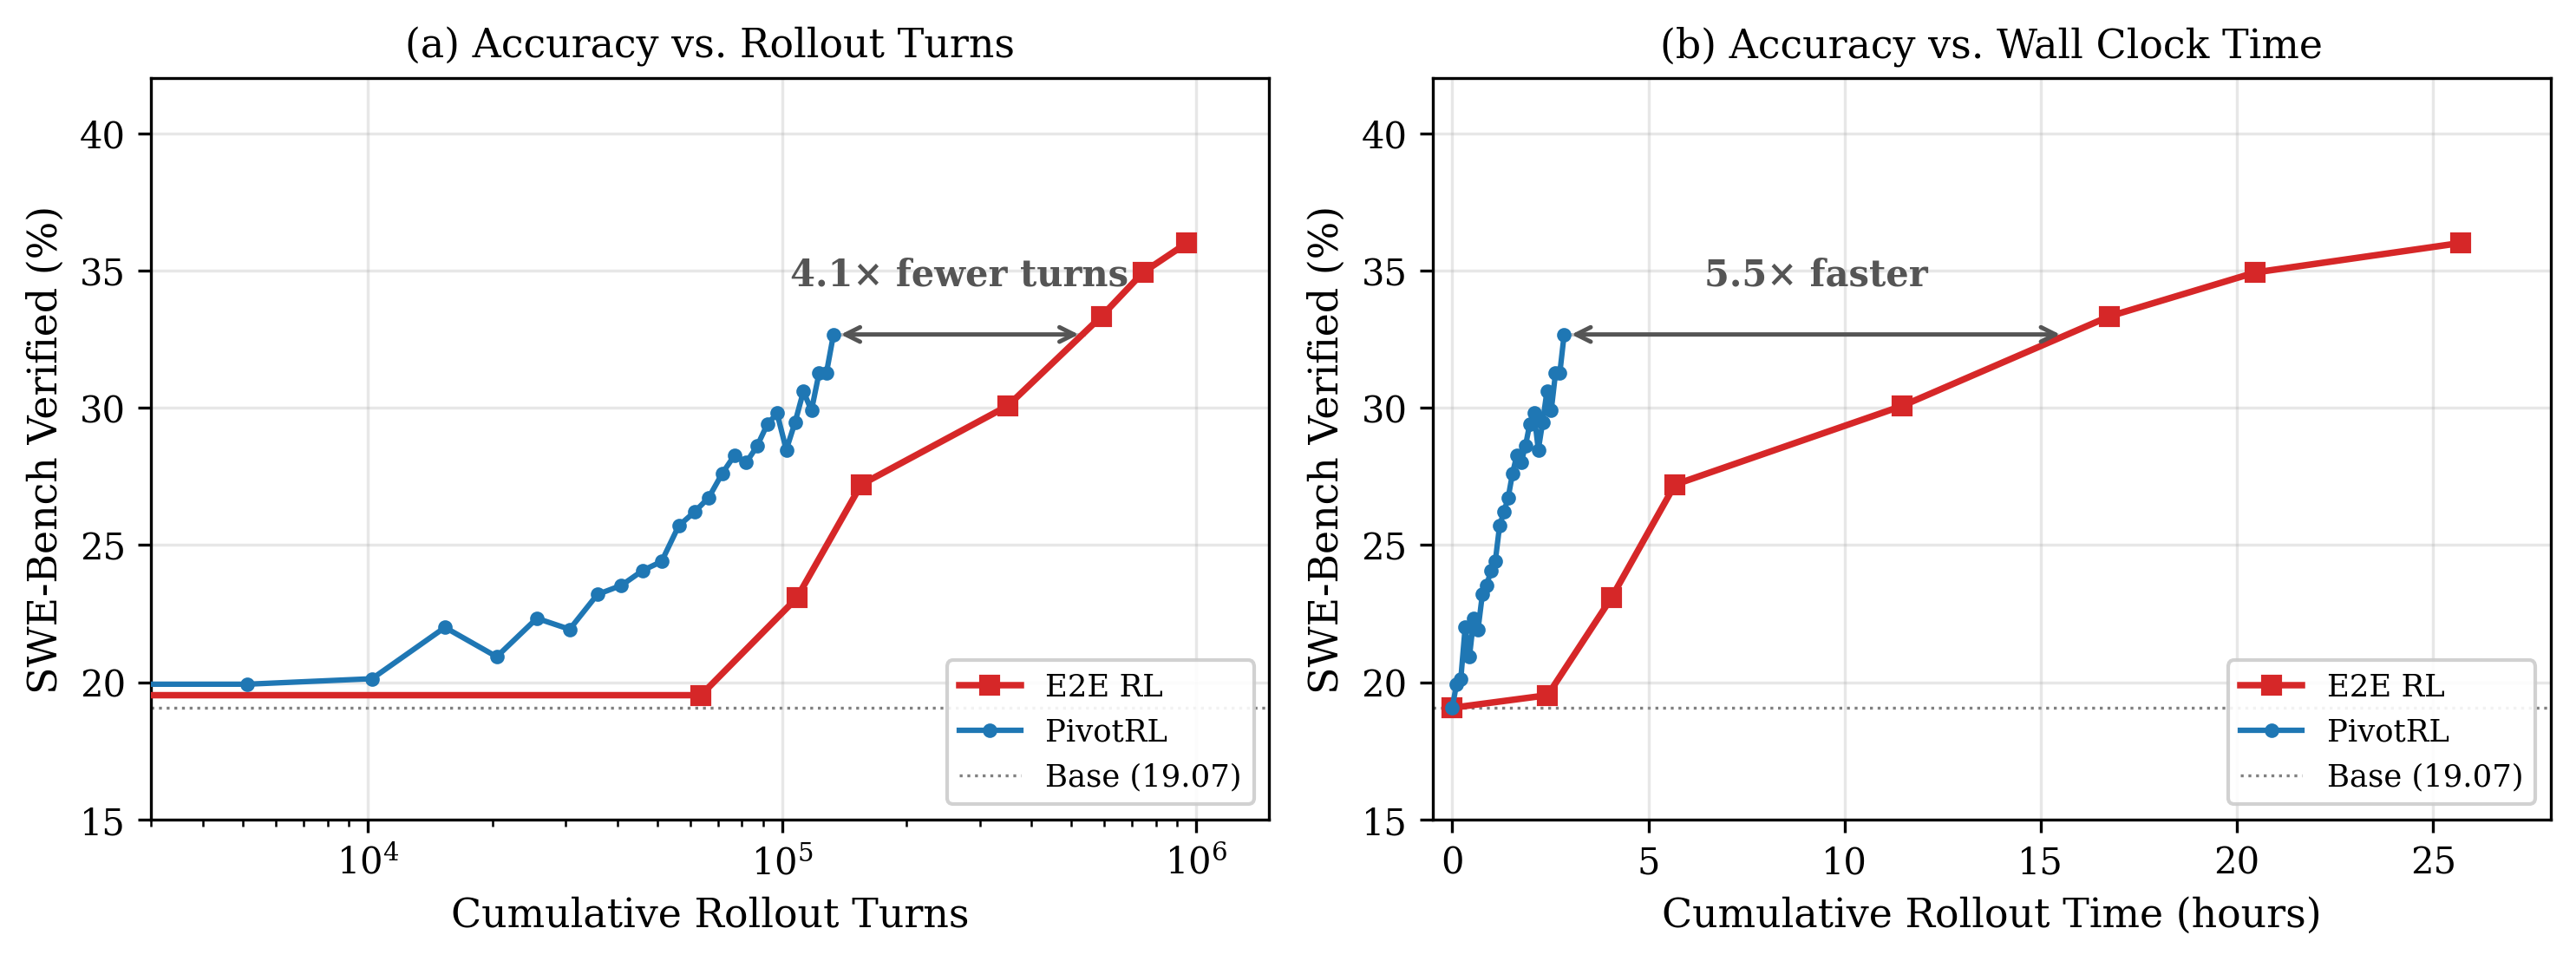
\includegraphics[width=\textwidth]{figures/swe_speedup_v2.png}
    \caption{SWE-Bench accuracy vs.\ (a) cumulative rollout turns and (b) cumulative rollout time during training, using the same number of compute nodes. PivotRL reaches comparable accuracy to E2E RL with ${\sim}4\times$ fewer rollout turns and ${\sim}5.5\times$ less wall-clock time.}
    \label{fig:swe_speedup}
\end{figure*}

%% ===================================================================
\subsection{Ablation Study}
\label{sec:ablation_study}

We present ablation results in Table \ref{tab:ablation_main}. To isolate the contribution of each PivotRL component, we remove one at a time on $\tau^2$-Bench.
\begin{table}[t]
\centering
\small
\begin{tabular}{lc}
\toprule
\textbf{Configuration} & \textbf{$\tau^2$-Bench} \\
\midrule
Full PivotRL ($\mathcal{D}_{\mathrm{adv}}$ + functional reward) & 63.81 \\
\quad $-$ Pivot filtering ($\mathcal{D}_{\mathrm{cand}}$ + functional reward) & 59.68 \\
\quad $-$ Functional reward ($\mathcal{D}_{\mathrm{cand}}$ + strict reward) & 57.34 \\
\midrule
Same-data SFT & 58.44 \\
Base & 44.35 \\
\bottomrule
\end{tabular}
\caption{
Ablation on $\tau^2$-Bench. Both pivot filtering and functional reward are necessary; removing either degrades accuracy.
}
\label{tab:ablation_main}
\end{table}
Removing filtering reduces accuracy from $63.81$ to $59.68$; removing functional reward yields $57.34$. Pivots concentrate rollouts on states with nonzero advantage signal (Proposition~\ref{prop:mixed}), and functional reward ensures that correct but textually different actions receive credit.

Figures~\ref{fig:tau_pivot_selection_acc} and~\ref{fig:tau_reward_std} show the training dynamics behind these gains. Under random sampling, per-batch reward variance collapses quickly, indicating that most sampled pivots no longer generate a useful advantage signal. The pivot sets preserve higher reward variance deeper into training and optimize to higher validation accuracy.

\begin{figure}[t]
    \centering
    \begin{minipage}{0.48\textwidth}
        \centering
        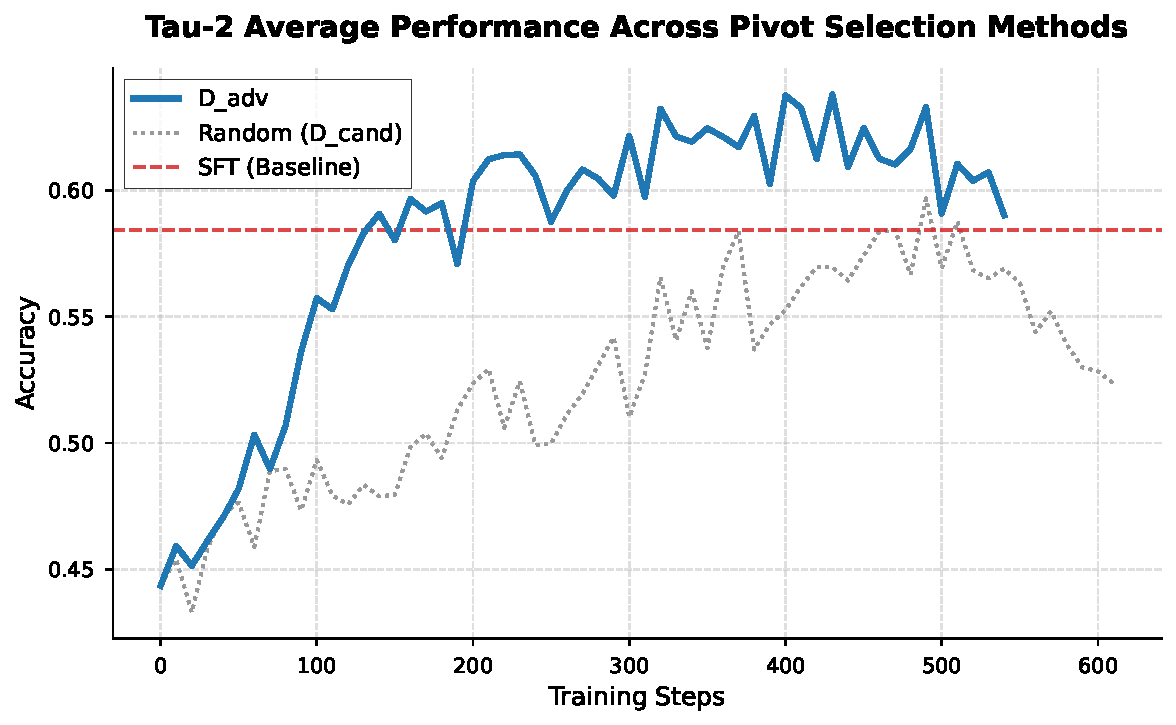
\includegraphics[width=\linewidth]{figures/main_average_validation.pdf}
        \caption{$\tau^2$-Bench accuracy over RL training. $\mathcal{D}_{adv}$ yields the strongest optimization and outperform same-data SFT.}
        \label{fig:tau_pivot_selection_acc}
    \end{minipage}
    \hfill
    \begin{minipage}{0.48\textwidth}
        \centering
        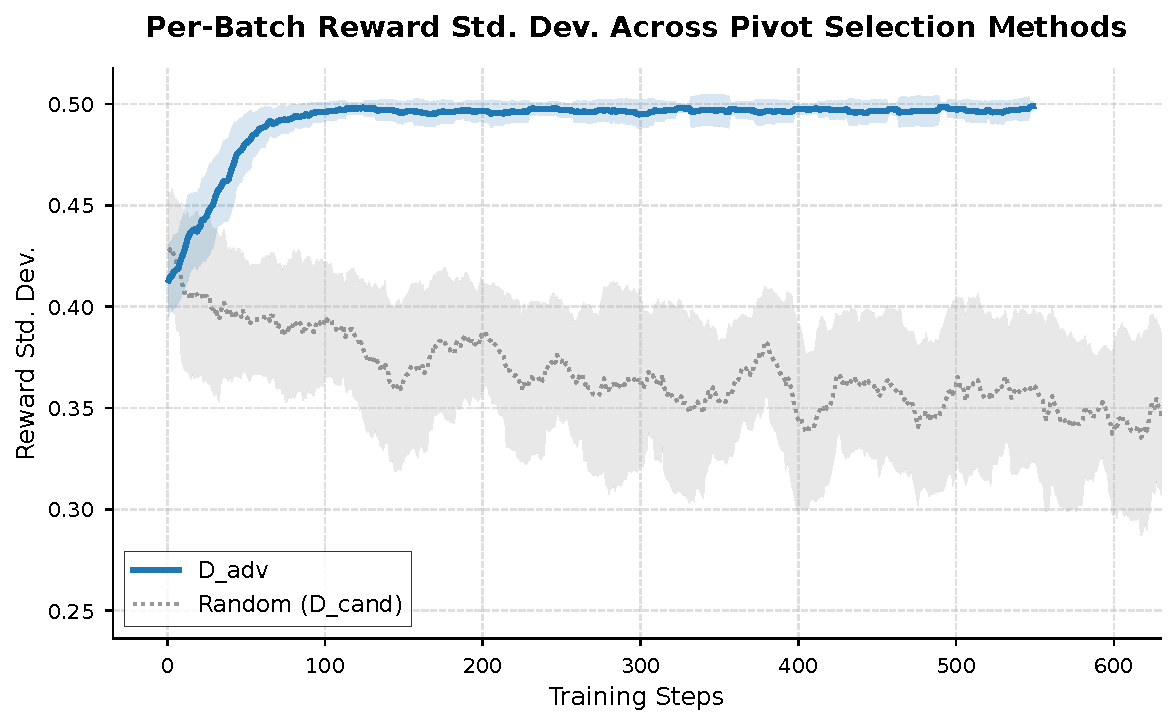
\includegraphics[width=\linewidth]{figures/tau_reward_stddev.pdf}
        \caption{$\tau^2$-Bench reward standard deviation during RL training. $\mathcal{D}_{adv}$ sets maintain higher reward variance and therefore more informative local updates.}
        \label{fig:tau_reward_std}
    \end{minipage}
\end{figure}






\subsection{Integration into Large-Scale Post-Training}
\label{sec:large_scale}

PivotRL was used during the large scale post training of Nemotron-3-Super \citep{nvidia2025nemotron3super}. Table~\ref{tab:large_scale_pivot} reports agentic benchmark accuracy during the Nemotron-3-Super post-training pipeline, where PivotRL covers the agentic environments while other RL environments handle reasoning and chat. 

\begin{table}[t]
\centering
\small
\begin{tabular}{lcc}
\toprule
\textbf{Benchmark} & \textbf{Nemotron-3-Super SFT} & \textbf{After PivotRL Stage} \\
\midrule
$\tau^2$-Bench         & 48.00 & 64.00 \\
SWE-Bench Verified     & 12.87 & 61.33 \\
Terminal-Bench 1.1 Core & 23.33 & 34.17 \\
BrowseComp             & 13.03 & 25.04 \\
\bottomrule
\end{tabular}
\caption{
Nemotron-3-Super agentic benchmark accuracy before and after the RL stage that included PivotRL environments for the agentic verticals and other RL environments for reasoning and chat. 
}
\label{tab:large_scale_pivot}
\end{table}
